
%(BEGIN_QUESTION)
% Copyright 2007, Tony R. Kuphaldt, released under the Creative Commons Attribution License (v 1.0)
% This means you may do almost anything with this work of mine, so long as you give me proper credit

Combustion heaters fired with a solid fuel such as coal often use {\it pulverizing mills} (sometimes called {\it ball mills}) to crush the coal into a powder for more efficient combustion.  The following is a P\&ID showing a fuel ``flow'' control system for such a solid fuel:

$$\includegraphics[width=15.5cm]{i01818x01.eps}$$

Solid coal from the hopper is weighed and fed by a variable-speed conveyor belt, then dumped into the ball mill where many steel balls tumbling in the cylindrical barrel of the mill grind the coal into smaller pieces, then carried into a ``cyclone'' separator where only the fine dust continues to the burner.  Coarser pieces falling out of the separator go back into the ball mill for additional pulverizing.  

Determine the purpose of the multiplying relay (FY) in this control system.  Hint: since the weight scale only measures the weight of a section of loaded conveyor belt, its output is expressed in units of pounds per foot (of belt).  The speed transmitter, of course, outputs a speed signal with units such as feet per minute (of belt).

\vskip 10pt

\filbreak

One problem with this control system is that the ball mill and cyclone separator introduce lag and dead time into the process.  That is, a sudden change in flow rate as detected by the weighfeeder conveyor equates to a delayed change in dust/air flow to the burner due to the time it takes for this additional fuel to make its way through the mill and separator.  A modification made to the control system helps avoid potential fuel flow control problems:

$$\includegraphics[width=15.5cm]{i01818x02.eps}$$

Explain how the addition of this lag function helps the flow controller (FC) do a better job of controlling fuel flow to the burner.

\vskip 20pt \vbox{\hrule \hbox{\strut \vrule{} {\bf Suggestions for Socratic discussion} \vrule} \hrule}

\begin{itemize}
\item{} Explain exactly how a ``cyclone'' separator does its job.
\end{itemize}

\underbar{file i01818}
%(END_QUESTION)





%(BEGIN_ANSWER)

The multiplier relay provides the flow controller with an actual {\it mass flow rate} signal for the coal.  The dead + lag time relay ``models'' the mill and separator, so that the flow controller sees a virtual representation of fuel flow going out the separator and to the burner.

\vskip 10pt

This ingenious application of lag and dead time function blocks in a control system provides an {\it inferred} variable of coal dust flow rate to the burners, where no suitable flowmeter exists to measure that quantity.  Measuring mass flow rate of coal chunks is easy with a weighfeeder, but extraordinarily difficult when the coal is in powdered form and fluidized by a moving air stream.  By adding the appropriate amount of lag time and dead time after the weighfeeder's mass flow signal, the flow controller ``sees'' the equivalent of powdered coal dust flow as it enters the burner, and so may be tuned to control this lagging and dead-timed quantity better than if it only ``saw'' the instantaneous flow rate of coal into the ball mill.

%(END_ANSWER)





%(BEGIN_NOTES)

Note: this control strategy derived from diagram on page 47 of Francis G. Shinskey's {\it Energy Conservation Through Control}, copyright 1978.

%INDEX% Process: coal fuel feed to combustion boiler
%INDEX% Process: pulverizing mill
%INDEX% Relay, computational: lag time used to model real process lag

%(END_NOTES)


